\newpage

\section{Programska podrška infotainment računala}

Infotainment računalo je Raspberry Pi 4 s DSI touchscreen zaslonom. 
Na njemu se izvodi prilagođena Linux distribucija izrađenu pomoću Yocto build sustava. 
Grafička aplikacija napisana je koristeći C++ i Qt programski okvir. Ova programska podrška nije glavni fokus ovog rada i neće biti detaljnije obrađena.

\begin{figure}[H]
  \begin{center}
    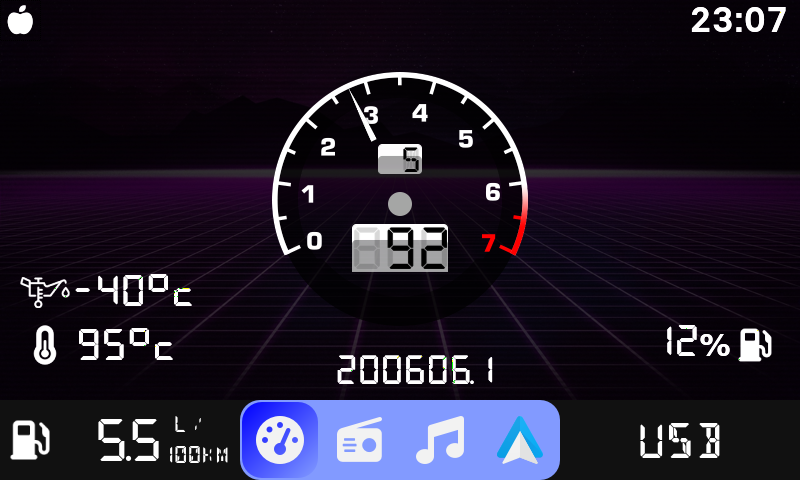
\includegraphics[width=0.75\textwidth]{images/1-rpm.png}
    \caption{Slika zaslona prethodne verzije programske podrške}
  \end{center}
\end{figure}

\noindent
Značajke:
\begin{itemize}
  \item Osnovna telemetrija u stvarnom vremenu (broj okretaja motora i temperatura, brzina vozila, stanje goriva)
  \item Informacije o vozilu (status vrata, putno računalo)
  \item Informacije o radiju (informacije o radio stanici, informacije o CD playeru)
  \item Lokalni glazbeni player
  \item Bluetooth player
  \item Kontrola svjetline zaslona ovisno o dobu dana
\end{itemize}